\documentclass[10pt, conference, compsocconf]{IEEEtran}
%IEEEtran
%acmart

\usepackage{flushend}
\usepackage{amsmath,amssymb,amsfonts}
\usepackage{algorithmic}
\usepackage{graphicx}
\usepackage{textcomp}
\usepackage{xcolor}
\usepackage{array}
\usepackage{subcaption}
\usepackage{listings}
\usepackage{color}
\usepackage{pdfpages}

\def\BibTeX{{\rm B\kern-.05em{\sc i\kern-.025em b}\kern-.08em
		T\kern-.1667em\lower.7ex\hbox{E}\kern-.125emX}}

\usepackage{listings}
\usepackage{color}

\definecolor{dkgreen}{rgb}{0,0.6,0}
\definecolor{gray}{rgb}{0.5,0.5,0.5}
\definecolor{mauve}{rgb}{0.58,0,0.82}

\lstset{frame=tb,
	language=Java,
	aboveskip=3mm,
	belowskip=3mm,
	showstringspaces=false,
	columns=flexible,
	basicstyle={\small\ttfamily},
	numbers=none,
	numberstyle=\tiny\color{gray},
	keywordstyle=\color{blue},
	commentstyle=\color{dkgreen},
	stringstyle=\color{mauve},
	breaklines=true,
	breakatwhitespace=true,
	tabsize=3
}


\begin{document}
\title{Predicting Co-Changes between Functionality Specifications and Source Code in Behavior Driven Development}

\author{\IEEEauthorblockN{Aidan Z.H. Yang}
	\IEEEauthorblockA{\textit{Electrical and Computer Engineering} \\
		\textit{Queen's University}\\
		Kingston, Ontario, Canada \\
		a.yang@queensu.ca}
	\and
	\IEEEauthorblockN{Daniel Alencar da Costa}
	\IEEEauthorblockA{\textit{Department of Information Science} \\
		\textit{University of Otago}\\
		Dunedin, Otago, New Zealand \\
		danielcalencar@otago.ac.nz}
	\and
	\IEEEauthorblockN{Ying Zou}
	\IEEEauthorblockA{\textit{Electrical and Computer Engineering} \\
		\textit{Queen’s University}\\
		Kingston, Ontario, Canada \\
		ying.zou@queensu.ca}
	}

\maketitle

\begin{abstract}
Behavior Driven Development (BDD) is an agile approach that uses \textit{.feature} files to describe the functionalities of a software system using natural language constructs (English-like phrases). Because of the English-like structure of \textit{.feature} files, BDD specifications become an evolving documentation that helps all (even non-technical) stakeholders to understand and contribute to a software project. After specifying a \textit{.feature} files, developers can use a BDD tool (e.g., Cucumber) to automatically generate test cases and implement the code of the specified functionality. However, maintaining traceability between \textit{.feature} files and source code requires human efforts. Therefore, \textit{.feature} files can be out-of-date, reducing the advantages of using BDD. Furthermore, existing research do not attempt to improve the traceability between \textit{.feature} files and source code files. In this paper, we study the co-changes between \textit{.feature} files and source code files to improve the traceability between \textit{.feature} files and source code files. Due to the English-like syntax of \textit{.feature} files, we use natural language processing to identify co-changes, with an accuracy of 79\%. We study the characteristics of BDD co-changes and build random forest models to predict when a \textit{.feature} files should be modified before committing a code change. The random forest model obtains an AUC of 0.77. The model can assist developers in identifying when a \textit{.feature} files should be modified in code commits. Once the traceability is up-to-date, BDD developers can write test code more efficiently and keep the software documentation up-to-date. 
\end{abstract}

%
% The code below should be generated by the tool at
% http://dl.acm.org/ccs.cfm
% Please copy and paste the code instead of the example below.
%

\begin{IEEEkeywords}Behavior Driven Development, Traceability, Co-Changes, Empirical Software Engineering
\end{IEEEkeywords}



\section{Introduction}

To reduce the communication barriers between development teams and customers, a new form of testing strategy, \textit{Behavior Driven Development} (BDD), became more prevalent in recent years \cite{solis2011study}. BDD aims to combine business and technical interests using a domain-specific language (DSL) that is similar to the English language. In BDD, the stakeholders specify \textit{scenarios} in \textit{.feature} files to describe functionalities of software. The scenarios can be described by all stakeholders of a project due to the simplistic English-like language format of BDD. The stakeholders can be customers, who have little to no programming experience, but can still define software requirements (or understand the logic of an implementation) using \textit{.feature} files. Because scenarios serve as a description of the functionality of a software, it is important to keep scenarios up-to-date as the functionalities of the software evolves. For example, when  a new developer arrives in a project, having the \textit{.feature} files up-to-date would ease the learning curve of the developer, i.e., the \textit{.feature} files would capture the most current functionalities in a friendly and precise manner.

The \textit{BDD co-changes} occur when a \textit{.feature} file and its corresponding source code files are modified in the same commit, or over different commits but in a close time span. As a BDD project scales up, the traceability of these co-changes may become harder to grasp because the links between \textit{.feature} files and their corresponding source code files naturally increase. An \textit{out-of-sync} BDD co-change occurs when a \textit{.feature} file and its corresponding source code files are modified in separate commits. The problem of maintaining BDD co-changes becomes more challenging when new developers enter into the project because they would have to identify the existing links between BDD files and source code files.


Existing research establishes the characteristics of BDD by studying large scale BDD projects in detail. Solís \textit{et al.} \cite{solis2011study} found that \textit{ubiquitous language} and \textit{Iterative Decomposition Process} are key characteristics of BDD. Other research work discussed the advantages of BDD in circuit design and verification \cite{diepenbeck2012behavior}. Regarding testing strategies, Bhat \textit{et al.} \cite{bhat2006evaluating} evaluated the efficiency of Test Driven Development (TDD), and Zaidman \textit{et al.} \cite{zaidman2008mining} explored the traceability of source and test code. With regards to co-changes, Mcintosh \textit{et al.} \cite{mcintosh2014mining} studied large scale software projects to predict co-changes between build system changes and source code changes. Although the characteristics of BDD and the traceability between test code and source code have been studied, maintaining the traceability between \textit{.feature} files and source code remains unexplored. Maintaining such traceability is important because it keeps the documentation (i.e., software scenarios) up-to-date, help developers learn the project faster, and better enforce the adopted testing strategy. We use an illustrative example in \textit{Section 2} to demonstrate the difficulty in maintaining \textit{.feature} files and source code file co-changes.

Our work aims to help developers identify when \textit{.feature} files should be modified before committing code. After mining and analyzing 133 GitHub projects that use BDD, we address the following three research questions:

\begin{itemize}
\item \textbf{(RQ1) Can we accurately identify co-changes between \textit{.feature} files and source code files?}

We link \textit{.feature} files and source code files by measuring the similarities between English phrases in \textit{.feature} and source code. After performing a manual analysis to evaluate the quality of the established links, we conclude that we can automatically identify co-changes between \textit{.feature} files and source code files with an accuracy of 79\%.

\item \textbf {(RQ2) Can we accurately predict when co-changes between \textit{.feature} files and source code files are necessary?}

To help developers determine the necessity of changing \textit{.feature} files before committing source code files, we identify the characteristics that can predict the modification of \textit{.feature} files within a commit. We use three classification techniques (random forest, Naive Bayes, and logistic regression) to predict corresponding \textit{.feature} file co-changes when changes in source code are made. Our random forest, Naive Bayes and logistic regression classifiers can predict \textit{.feature} file co-changes with a relatively high AUC of 0.77, 0.74, and 0.70, respectively.

\item \textbf {(RQ3) What are the most significant characteristics for predicting co-changes between \textit{.feature} files and source code files?}

To identify the characteristics that are most important to predict co-changes between \textit{.feature} files and source code files, we analyze the classification technique with the highest AUC (i.e., our random forest technique). We use a mean decrease AUC approach on the random forest classifier to identify the most important characteristics to predict co-changes between \textit{.feature} file and source code files. We observe that \textit{test files added} and \textit{source LOC deleted} are the most influential characteristics.

\end{itemize}

The remainder of the paper is organized as follows. In \textit{Section 2}, we provide a motivating example to our work. \textit{Section 3} outlines the experiment setup. \textit{Section 4} presents the results with respect to our three research questions, and \textit{Section 5} discusses threats to the validity of our results. In \textit{Section 6}, we examine related work and \textit{Section 7} draws conclusions to the paper.






\section{Motivating Example}
We study the \textit{Trivial-Graph} \cite{akollegger_2011} GitHub project to demonstrate the importance of maintaining the traceability between \textit{.feature} files and source code files. \textit{Trivial-Graph} is a web-based trivia game application in which teams compete to answer questions in multiple rounds. \textit{Trivial-Graph} uses the \textit{Cucumber} BDD framework \cite{akollegger_2011, BDDFrame} to write \textit{.feature} files and \textit{step definition} files. The \textit{.feature} files describe the scenarios (i.e., functionalities) of the project. The \textit{step definition} files are automatically generated by \textit{Cucumber} based on the \textit{.feature} files. The \textit{step definition} files define the tests for the functionalities specified in the \textit{.feature} files. 
Figure 1 shows an example of a \textit{.feature} file and its corresponding \textit{step definition} file. A \textit{step definition} file has annotations (e.g., ``@When" and ``@Then") to indicate which step of a \textit{.feature} file is tested by a given test method. The developer then runs the tests on the source code using the \textit{step definition} files, until every tests passes, satisfying the functions of each scenario

\begin{figure}
	\textbf{\textit{.feature} file code}:
	\begin{lstlisting}
	@players
	Feature: Trivialt Players and Teams
	Scenario: Register as a new player
	When you register "Tobias" with handle "@thobe"
	Then trivialt knows "@thobe" is "Tobias"
	And "@thobe" should be the current player
	\end{lstlisting}
	\textbf{Step definition file code}:
	\begin{lstlisting}
	@players
	@When("^you register \"([^\"]*)\" with handle \"([^\"]*)\"$")
	public void youRegisterUser(String name, String handle){
		currentPlayer = trivialtWorld.register(handle, name);
		assertThat(currentPlayer, is(not(nullValue())));
	}
	@Then("^trivialt knows \"([^\"]*)\" is \"([^\"]*)\"$")
	public void trivialtKnowsPlayer(String handle, String name){
	        Player foundPlayer = trivialtWorld.findPlayer(handle);
			assertThat(foundPlayer, is(not(nullValue())));
			assertThat(foundPlayer.getName(), is(name));
	}
	 @Then("^\"([^\"]*)\" should be the current player$")
	public void assertTheCurrentPlayerIs(String handle){
		assertThat(currentPlayer.getHandle(), is(handle));
	}
	\end{lstlisting}
	\caption{Code example from BDD files}
	
\end{figure}

\begin{figure*}
	\centering
	\includegraphics[height=4.7in, width=6.5in]{timeline.pdf}
	\caption{Time line of an example BDD project}
\end{figure*} 
We observe co-changes between \textit{.feature} files and source code files in the \textit{Trivial-Graph} by studying six commits in a one month time frame during 2011 (shown in Figure 2). Figure 2 shows an out-of-sync co-change in the dotted lines surrounding commits 4 and 5. In commit 1, the author creates the project. A week later, the author adds the \textit{app.feature} file in commit 2 as well as the corresponding source code files. Similarly, in commit 3, the author adds the \textit{team\_players.feature} file and the corresponding source code files (i.e., Add \textit{Teams.java} and \textit{Players.java}). The author then follows the requirements described by \textit{app.feature} and \textit{team\_players.feature} to add LOC in App.java and \textit{Players.java} in commit 4. However, in commit 4, the author does not modify \textit{.feature} files to describe the newly added source code functionalities. Roughly two hours later, in commit 5, the author adds LOC to \textit{app.feature} and \textit{team\_players.feature} and writes the following commit message ``Added missing steps". In each of these commits, we observe co-changing \textit{.feature} files and source code files (i.e., \textit{app.feature} co-changing with \textit{App.java}, and team\_players.feature co-changing with \textit{Players.java}). However, the co-changing files are not modified simultaneously. We identify \textit{.feature} file co-changes across different commits, i.e., source code files in commit 4 co-changing with \textit{.feature} files in commit 5. We observe that, although\textit{ app.feature} and \textit{AppTest.java} are co-changing files, the author does not include \textit{app.feature} changes in commit 4, showing a temporary \textit{out-of-sync} co-change. As a result of this out-of-sync co-change, the author needs to make another commit roughly two hours after commit 4. After step 6, we observe that \textit{app.feature} is modified with \textit{AppTest.java} in the same commit frequently, showing a continuing co-change link between the two files.

As the project scales up, it becomes harder to understand which \textit{.feature} file corresponds with which source file or methods, and out-of-sync co-changes become more prevalent. In commit 5 of Figure 2, we observe that \textit{team\_players.feature} correspond to three different source files, and the \textit{.feature} file is still modified 18 days after its first co-changing source file was added. As the project grows larger, the \textit{.feature} file will need to be modified to describe functionalities of other source files, causing the \textit{.feature} file maintenance time even longer. For a developer joining such a project, it is time-consuming and challenging to identify every co-change between \textit{.feature} files and source code files. We explore approaches that can ease the traceability of co-changes between \textit{.feature} files and source code files and reduce the out-of-sync co-changes. 


\section{Experiment Setup}
\begin{figure*}
	\centering
	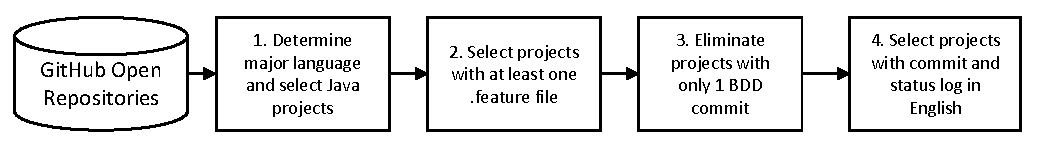
\includegraphics[height=0.9in, width=6.6in]{exp_setup.pdf}
	\caption{An overview of the experiment design}
\end{figure*}
In this section, we explain how we collect the data used for answering our research questions.

Figure 3 shows an overview of our entire experiment setup process. In \textbf{Step 1}, we use the GitHub search API to find project that mainly uses Java. We choose Java because the BDD framework \textit{Cucumber} for Java is currently the most popular BDD tool \cite{BDDFrame}. Filtering Java projects is done by the search API of GitHub. Using the API, we can identify the major language of a project. GitHub uses the \textit{Linguist} library to identify the major language in each project. Our search retrieves 1,005,247 projects in total and we extract 59,933 Java projects amongst all the retrieved projects. In \textbf{Step 2}, we use the tree API in GitHub to find projects that include at least one \textit{.feature} file, which we deem as a BDD project. We find that 927 out of 59,933 projects actually contain \textit{.feature} files. In \textbf{Step 3}, we filter out the projects that contain only one commit manipulating a \textit{.feature} file to avoid projects that do not actually use BDD. After this filtering, 890 projects survive. In \textbf{Step 4}, we eliminate BDD projects that do not have both \textit {commit log} and \textit {status} data in English. Commit logs provide information regarding every modification to the project (e.g., why certain files are modified). The status data stores the status of every commit, i.e., author, date and modified files. For our research, it is important for the information to be in English to understand the purpose of each commit and to make our research more reproducible. Also, we perform text processing with regards to English words in RQ1, so projects with information in a foreign language (e.g., Arabic) would hinder our analyses. In the end, 133 BDD projects remain. We highlight some key characteristics of our studied projects by selecting 50 of our 133 BDD projects with the highest total LOC. Table 1 shows the year created, total commits, total pull requests, total forks and total stars for each of our studied projects.

\begin{table*}
	\normalsize
	\caption{Characteristics of 50 studied BDD projects}
	\center
	
	\begin{tabular}{p{6cm} c c c c c}
		\textbf{Project} (Username/Project-Name) & \textbf{Year Created} & \textbf{Total commits} & \textbf{Pull requests} & \textbf{Forks} & \textbf{Stars}\\
		\hline
tyen/cs320tests & 2009 & 207 & 0 & 0 & 9 \\
caspian311/Scripturelookup & 2009 & 109 & 0 & 0 & 2 \\
epabst/expressive & 2009 & 72 & 0 & 1 & 3 \\
epabst/expressiveBDD & 2009 & 46 & 0 & 2 & 2 \\
mkristian/slf4r & 2009 & 41 & 0 & 0 & 6 \\
Vaysman/jvote & 2009 & 29 & 0 & 0 & 0 \\
Serabe/javascreepy & 2009 & 22 & 0 & 0 & 1 \\
rapidftr/RapidFTR-Android & 2010 & 1214 & 31 & 83 & 38 \\
davidbkemp/nate & 2010 & 259 & 0 & 0 & 0 \\
jtigger/kanban-simulator & 2010 & 196 & 0 & 0 & 4 \\
yujunliang/lambda & 2010 & 83 & 0 & 0 & 8 \\
jacek99/maven-python-mojos & 2010 & 73 & 1 & 12 & 18 \\
rapaul/cuke4ninja & 2010 & 70 & 0 & 0 & 1 \\
trevershick/jook & 2010 & 69 & 2 & 2 & 1 \\
sveinung/pritest-server & 2010 & 57 & 1 & 0 & 6 \\
openengsb-labs/labs-yaste & 2010 & 32 & 0 & 1 & 3 \\
runeflobakk/poker & 2010 & 27 & 0 & 1 & 1 \\
bugsnag/bugsnag-android & 2011 & 645 & 29 & 154 & 872 \\
AndreasWilhelm/neo4j-spatial & 2011 & 360 & 0 & 0 & 2 \\
resthub/springmvc-router & 2011 & 214 & 29 & 59 & 170 \\
rlogiacco/SmartUnit & 2011 & 178 & 5 & 5 & 15 \\
vitormcruz/payroll\_cs & 2011 & 173 & 0 & 0 & 2 \\
mkristian/rails-resty-gwt & 2011 & 164 & 0 & 2 & 12 \\
akollegger/trivial-graph & 2011 & 85 & 0 & 0 & 1 \\
jfinkhaeuser/androdyne & 2011 & 64 & 0 & 0 & 5 \\
Drin/spam & 2011 & 50 & 0 & 1 & 1 \\
dokipen/embedly-java & 2011 & 39 & 1 & 9 & 1 \\
jescov/jescov & 2011 & 39 & 0 & 4 & 10 \\
jkransen/treemarks & 2011 & 38 & 0 & 0 & 0 \\
Jennifer-fu/practices & 2011 & 36 & 0 & 0 & 1 \\
lukasz-kaniowski/cucumber-selenium-rc & 2011 & 33 & 0 & 1 & 2 \\
ZsoltFabok/cucumber-jvm-post & 2011 & 22 & 0 & 10 & 17 \\
Chorus-bdd/Chorus & 2012 & 1124 & 17 & 9 & 35 \\
bartbaas/spatial & 2012 & 565 & 0 & 0 & 2 \\
daniel-andersen/Q-Cumberless-Testing & 2012 & 348 & 0 & 0 & 4 \\
leviwilson/oasis-android & 2012 & 244 & 0 & 0 & 1 \\
tlauchenauer/gaia-pdb & 2012 & 237 & 0 & 0 & 1 \\
bclozel/springmvc-router & 2012 & 214 & 2 & 7 & 42 \\
rabid-fish/JavaTechExamples & 2012 & 178 & 0 & 0 & 1 \\
iantmoore/old-substeps-webdriver & 2012 & 163 & 0 & 1 & 1 \\
ericlemerdy/one-kata-per-day & 2012 & 118 & 0 & 3 & 7 \\
mikael-wilhelm/LoadPlannerAmaz & 2012 & 109 & 0 & 0 & 1 \\
marky-mark/MTT & 2012 & 77 & 0 & 0 & 1 \\
leefaus/soa-petstore & 2012 & 56 & 0 & 4 & 4 \\
suggitpe/java-web & 2012 & 40 & 0 & 1 & 0 \\
japonophile/jescov & 2012 & 39 & 0 & 0 & 1 \\
sandromancuso/tww-java & 2012 & 33 & 0 & 0 & 2 \\
ilanpillemer/gherkin-eclipse-plugin & 2012 & 26 & 0 & 2 & 18 \\
talios/cucumber-testng-factory & 2012 & 26 & 3 & 9 & 13 \\
hayatoshimizuBSKYB/apollo & 2012 & 23 & 3 & 1 & 5

	\end{tabular}
\end{table*}

\input{RQ1}
\input{RQ2}
\input{RQ3}
\input{threats}
\input{related_works}
\section{Conclusions}
BDD is a relatively new testing strategy that uses English-like syntax in describing code functionalities. BDD makes it easier for all stakeholders involved in a project to understand the functionalities of a software project. With the use of \textit{.feature} files in describing the functionalities of a software, the co-evolution of \textit{.feature} files and source code files must be kept up-to-date. In our work, we detect the co-changes between \textit{.feature} files and source code files, and find characteristics that can accurately predict the co-changes in order to improve the traceability between \textit{.feature} files and source code files.

Our approach can link \textit{.feature} files with source code files with an accuracy of 79\% and predict co-changes between \textit{.feature} files and source code files with an AUC of 0.77. \textit{Test files added}, \textit{other files modified}, \textit{test files renamed}, and \textit{source LOC deleted} are the best predictors for co-changes between \textit{.feature} files and source code files. Our results demonstrate that co-changes between \textit{.feature} files and source code files can be detected, and that source code change characteristics can predict those co-changes. Our findings can help developers to keep software documentation (i.e., \textit{.feature} files) up-to-date and help projects to adopt the BDD practices in developing software more efficiently. To further assist BDD developers, we plan to explore BDD co-changes with regards to more languages and analyze more projects using BDD.




\bibliographystyle{ieeetran}
%ieeetran
%apacite
\bibliography{references}


\end{document}
